\documentclass[12pt]{article}

\usepackage{fontawesome}
\usepackage{hyperref}
\usepackage{xurl}
\usepackage{graphicx}
\usepackage{float}
\usepackage[tagged, highstructure]{accessibility}
\usepackage{bookmark}
\usepackage{enumitem}

\hypersetup{
    colorlinks=false,
    pdfborder={0 0 0},
    pdftitle={Social Engineering},
    pdfauthor={Adrianna Holden-Gouveia},
    pdfsubject={Information Security - Lab Assignment},
    pdflang={en-US},
    pdfkeywords={social engineering, human behavior, security awareness, body language}
}

% Configure PDF bookmarks for navigation
\bookmarksetup{
    numbered,
    open,
}

% Configure list spacing for better accessibility
\setlist{nosep}



\title{Social Engineering}
\author{
        Adrianna Holden-Gouveia \\
        Website: \href{https://aholdengouveia.name}{aholdengouveia.name}\\ 
        \date{\vspace{-5ex}}
        %Email: \href{mailto:admin@aholdengouveia.name}{admin@aholdengouveia.name} \\
%        \faLinkedin{: aholdengouveia} \\
        \faGithub {: aholdengouveia} \\
        \faTwitter {: aholdengouveia} \\
        }

%S\date{\today}


\begin{document}    

\maketitle

\section*{Accessibility Notice}
This document is also available in HTML format at:

Link: \href{https://aholdengouveia.name/InfoSec/labs/socialengineering.html}{\textbf{\nolinkurl{https://aholdengouveia.name/InfoSec/labs/socialengineering.html}}}

The HTML version provides enhanced accessibility features including keyboard navigation, screen reader support, responsive design, dark mode support, and high contrast options.


%\begin{abstract}
%This is a template for Linux Administration Lab work
%\end{abstract}
%\tableofcontents

As we do these activities, remember these rules.
\begin{enumerate}
    \item Don't make anyone feel victimized or targeted.
    \item Treat information gathered in an ethical manner. 
    \item Don't break any laws. 
    \item Don't abuse this knowledge. 
\end{enumerate}

    
    


\section*{Learning Outcomes}
By the end of this lab, you will be able to:
\begin{itemize}
    \item Identify social engineering attacks and the human behaviors they exploit, using real examples
    \item Analyze body language and dominance in conversations you observe
    \item Recommend ways a person can protect themselves from social engineering
\end{itemize}

\section*{Lab Instructions}
\subsection*{Part 1: Real-World Examples}
Find and describe two real-world examples of social engineering attacks. Explain how each attack exploited human behavior to compromise security. Your examples can be from the news or something you saw in person. Recent attacks that used AI, such as deepfake video calls or tricking an AI support chatbot, are good choices.

For each example from the news, include your source with the following. My guide to evaluating sources, linked under Resources, shows how to do the CRAAP test, with a good and a bad example.
\begin{enumerate}
    \item A citation, and a CRAAP test checklist or paragraph: Currency, Relevance, Authority, Accuracy, and Purpose.
    \item A screenshot of the source, showing its title and date.
    \item One direct quote from the source, and where it appears, such as the paragraph or section.
\end{enumerate}

\subsection*{Part 2: Observation Game}
The way people greet and talk to each other says a lot about who feels dominant. For example, when someone shakes your hand and turns their hand so it's on top of yours, they're showing dominance. So is grabbing your upper arm during a handshake, or touching your arm or shoulder.

Watch at least 3 conversations. You don't need to hear what's said:
\begin{itemize}
    \item 1 between family members or friends you know well
    \item 1 between strangers
    \item 1 of either kind
\end{itemize}
If you don't have a safe way to watch conversations in person, watch a show or movie instead. Watch at least 30 minutes on mute for each conversation, or listen to something in a language you don't speak. Pick a drama or comedy with lots of people talking, such as a Shakespeare or Jane Austen remake like Hamlet or Pride and Prejudice. No animated videos, and action movies won't work well.

\textbf{Don't be creepy.} Social engineers watch people, and you're practicing the same skill, so do it respectfully:
\begin{itemize}
    \item Only watch people you know, or people in public places, from a normal distance.
    \item Don't follow anyone, stare, or listen in on private conversations.
    \item Don't take photos, video, or audio recordings of anyone.
    \item Don't write down names, or anything else that could identify a stranger.
    \item If someone notices you and seems uncomfortable, stop and move on.
\end{itemize}

\textbf{Body language checklist.} Use my body language checklist, linked under Resources, to guide what you look for. It has examples for handshakes, posture, eye contact, touch, personal space, talking, position, facial expressions, gestures, mirroring, feet, and tone. Read its notes first: body language is a clue, not proof, and people's culture, disability, and comfort all change how they move.

For each conversation, write down the date, the time, and the general setting, such as ``campus café, Tuesday afternoon'' or the name of the show and episode. Then answer:
\begin{enumerate}
    \item Was it a happy conversation? Sad? Tense? What led you to that conclusion?
    \item Which items from the body language checklist did you see? Describe them.
    \item Who was dominant during the conversation? Did dominance switch?
    \item Could you see facial expressions? What did you see, and what do you think they meant?
\end{enumerate}

\subsection*{Part 3: Video}
Watch the 60 Minutes segment on how con artists use AI and apps to steal (linked under Resources, with a transcript). An ethical hacker uses an AI copy of a reporter's voice to trick a coworker, and a family describes a grandparent scam. Answer these questions:
\begin{enumerate}[start=5]
    \item What information did the hacker find before making the call, and where did she find it?
    \item What made the call believable? Which human behaviors did it take advantage of, such as trust, helpfulness, or rushing?
    \item What could the coworker, or the grandparent, have done differently? What should they do in the future?
    \item What are 2 resources you would recommend to them? Include the full links.
\end{enumerate}

\subsection*{Screenshots}
Each screenshot should have your name, term, and year.  One of the easiest ways to do that is make a text document with your name and term/year on your computer and save it to use all term. Any screenshots that don't include this information won't be counted.

\begin{figure}[H]
    \centerline{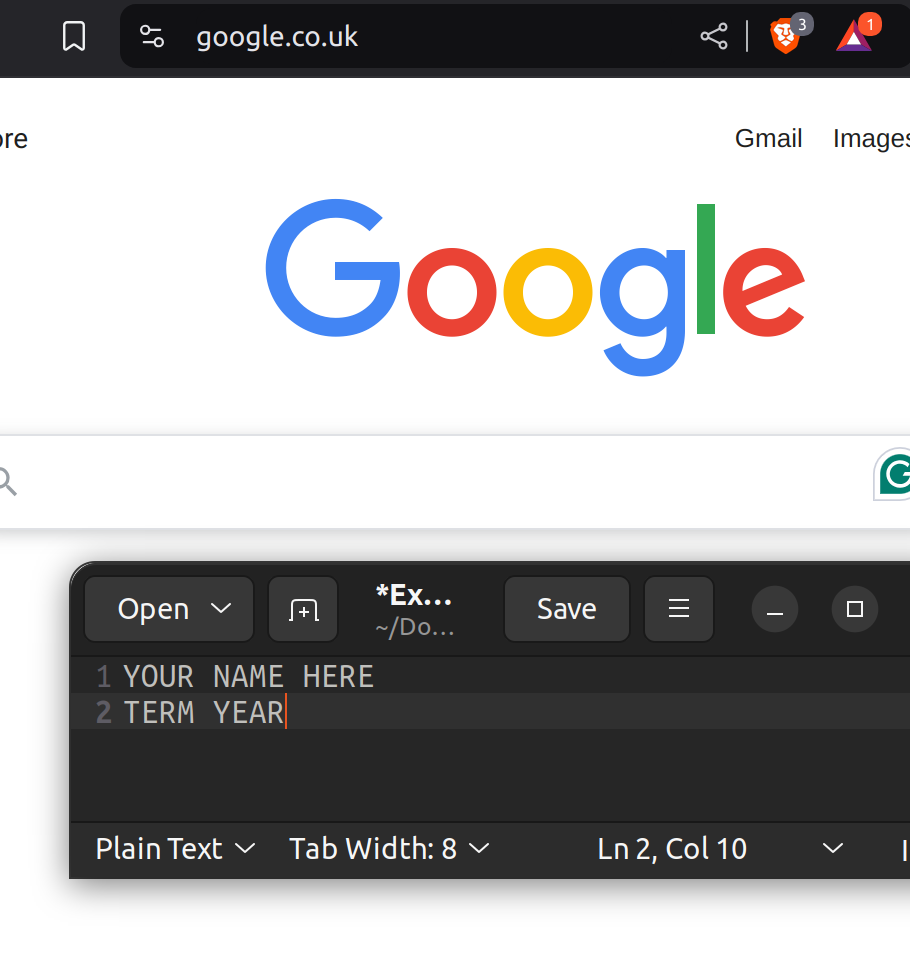
\includegraphics[scale=.2]{ExampleScreenshot.png}}
    \caption{This is an image of what each of your screenshots should look like}
    \alt{Example screenshot: a web browser showing the Google home page, with a small text editor window in front of it that says YOUR NAME HERE and TERM YEAR}
\end{figure}

\section*{Deliverables}
One file that includes:
\begin{itemize}
    \item Part 1: your 2 real-world examples, with a citation, CRAAP check, screenshot, and quote for each news source
    \item Part 2: your notes on all 3 conversations, each with the date, time, and setting, and your answers to the 4 questions
    \item Part 3: your answers to the 4 video questions
\end{itemize}
Explain why you think what you think. Even if you're pretty sure of an answer, include a source that agrees with you.

\section*{Resources}
References, a video, a PowerPoint and some notes are available at my website
Link: \href{https://www.aholdengouveia.name/InfoSec/DoSandSocialEngineering.html}{\textbf{\nolinkurl{https://www.aholdengouveia.name/InfoSec/DoSandSocialEngineering.html}}}

My body language checklist, for Part 2
Link: \href{https://www.aholdengouveia.name/InfoSec/labs/bodylanguage.txt}{\textbf{\nolinkurl{https://www.aholdengouveia.name/InfoSec/labs/bodylanguage.txt}}}

60 Minutes (CBS News, 2023): Con artists using AI, apps to target parents, grandparents for theft, the video for Part 3
Link: \href{https://www.youtube.com/watch?v=z9zaMw6VLJg}{\textbf{\nolinkurl{https://www.youtube.com/watch?v=z9zaMw6VLJg}}}

The transcript of the 60 Minutes segment
Link: \href{https://www.cbsnews.com/news/how-con-artists-use-ai-apps-to-steal-60-minutes-transcript/}{\textbf{\nolinkurl{https://www.cbsnews.com/news/how-con-artists-use-ai-apps-to-steal-60-minutes-transcript/}}}

My guide to evaluating sources
Link: \href{https://www.aholdengouveia.name/Howtos/Sourceeval/sourceEvaluation.html}{\textbf{\nolinkurl{https://www.aholdengouveia.name/Howtos/Sourceeval/sourceEvaluation.html}}}

The CRAAP test, with questions to ask about each source
Link: \href{https://web.archive.org/web/20250814000638/https://guides.lib.uchicago.edu/c.php?g=1241077&p=9082343}{\textbf{\nolinkurl{https://web.archive.org/web/20250814000638/https://guides.lib.uchicago.edu/c.php?g=1241077&p=9082343}}}

Another explanation of the CRAAP test
Link: \href{https://libguides.butler.edu/c.php?g=117303&p=1940068}{\textbf{\nolinkurl{https://libguides.butler.edu/c.php?g=117303&p=1940068}}}

\end{document}